\chapter[Heteroatomic Noble Gas Clusters]{Competing Processes in Heteroatomic Noble Gas Clusters}
\label{chapter_clusters}

The modelling of secondary electron spectra originating from \ac{ICD}
and \ac{ETMD}3 processes are carried out using the program
HARDRoC \cite{HARDRoC}. It is based on the model of pairs and
triples explained in chapter \ref{chapter:geom} and is applied
to a given cluster structure. The 
decay widths obtained are proportional to the probability of the underlying decay.
The experimental spectra are obtained from a multitude of distinct measurements.
Hence, for a reasonable large number of measurements, a distribution with the
same statistical behaviour as for the decay width calculation in the
model of pairs and triples is achieved. Therefore, the experimental spectra
can be directly compared with the theoretically obtained spectra.

The energies of the secondary electrons are calculated using
equation \ref{equation:E_sec}. The single ionization energies
can be obtained in two different ways. They can be
estimated by the atomic ionization energies in Table
\ref{table:noble_atom_properties} corrected by energetic shifts
given in Table \ref{table:cluster_shifts} in order to take
the effect of the cluster environment into account. 
Alternatively, their source can be the single ionization spectra measured
at the same time and the
same conditions as the electron-electron
coincidence experiment. The latter apporach is to be preferred,
since the energy shifts
of Table \ref{table:cluster_shifts} are obtained from analysis of
homonuclear cluster's ionization spectra and
hence the values only give a first approximation to the real energetic shift in
heteronuclear cluster. Since both, the \ac{ICD} and primarily the
\ac{ETMD}3 occur at interfaces, it is crucial for a good modelling to
describe the ionization energies of these atoms as accurate as possible.

The decay widths $\Gamma$ can either be obtained from the asymptotic expressions
in equations (\ref{reltheolifetime_exp}) and (\ref{reltheolifetimeetmd_exp})
using the atomic properties given in Table \ref{table:noble_atom_properties}
or from a fit to decay widths obtained from FanoADC-Stieltjes calculations.

In the following sections two different heteronuclear clusters are investigated
illustrating different effects on the secondary electron spectra.
In the case of ArXe clusters, the focus is set on the investigation of how
spin-orbit coupling affects
the secondary electron spectra. Furthermore, I will investigate the influence
of the cluster size and number of argon shells around the xenon core and
the effects of of the basic structure of the cluster and discuss the
difference between the spectra
obtained from clusters having an icosahedral
and \ac{fcc} structure.
In the case of NeAr clusters I will focus on the bidirectional dependence of
the ICD spectra of the competing NeNe-ICD and NeAr-ICD processes and
different arrangements of neon atoms around the argon core.

\newpage

\begin{figure}
 \centering
 \begin{tikzpicture}[scale=1.0]

\begin{axis}[%scale=1.5,
             domain=0:7,
             restrict expr to domain={x}{0:7},
             %restrict expr to domain={y}{1.0E-12:7},
             xlabel={E [eV]},
             %xtick={30,50,...,170},
             %xticklabels={2,4,6,8,10,12,15,20,25},
             %ytick={-1.0,-0.8,...,1.0},
             %yticklabels={1.0,0.8,0.6,0.4,0.2,0.0,0.2,0.4,0.6,0.8,1.0},
             ylabel={$\Gamma$ [eV]},
             scale only axis,
             width=\textwidth-1.5cm,
             height=8cm,
             %ybar stacked
             ]

%ICD
\addplot+[ycomb,
         mark=.,
         very thick,
         Green,
         forget plot
        ]
        table[
        x expr = \thisrowno{0},
        y expr = \thisrowno{4}
        ]
        {data/exp_309ico_icd_arxe.dat};
        \addlegendimage{line legend, Green, very thick};
        \addlegendentry{Ar$_{3/2}$ Xe$_{3/2}$};

\addplot+[ycomb,
         mark=.,
         very thick,
         Goldenrod,
         forget plot
        ]
        table[
        x expr = \thisrowno{0},
        y expr = \thisrowno{2}
        ]
        {data/exp_309ico_icd_arxe.dat};
        \addlegendimage{line legend, Goldenrod, very thick};
        \addlegendentry{Ar$_{1/2}$ Xe$_{3/2}$};

\addplot+[ycomb,
         mark=.,
         very thick,
         LimeGreen,
         forget plot
        ]
        table[
        x expr = \thisrowno{0},
        y expr = \thisrowno{3}
        ]
        {data/exp_309ico_icd_arxe.dat};
        \addlegendimage{line legend, LimeGreen, very thick};
        \addlegendentry{Ar$_{3/2}$ Xe$_{1/2}$};

\addplot+[ycomb,
         mark=.,
         very thick,
         Fuchsia,
         forget plot
        ]
        table[
        x expr = \thisrowno{0},
        y expr = \thisrowno{1}
        ]
        {data/exp_309ico_icd_arxe.dat};
        \addlegendimage{line legend, Fuchsia, very thick};
        \addlegendentry{Ar$_{1/2}$ Xe$_{1/2}$};

%ETMD
\addplot+[ycomb,
         mark=.,
         very thick,
         diplom1,
         forget plot
        ]
        table[
        x expr = \thisrowno{0},
        y expr = \thisrowno{4}
        ]
        {data/exp_309ico_etmd_arxe.dat};
        \addlegendimage{line legend, diplom1, very thick};
        \addlegendentry{Xe$_{3/2}$ Xe$_{3/2}$};

\addplot+[ycomb,
         mark=.,
         very thick,
         orange,
         forget plot
        ]
        table[
        x expr = \thisrowno{0},
        y expr = \thisrowno{2}
        ]
        {data/exp_309ico_etmd_arxe.dat};
        \addlegendimage{line legend, orange, very thick};
        \addlegendentry{Xe$_{1/2}$ Xe$_{3/2}$};

\addplot+[ycomb,
         mark=.,
         very thick,
         diplom2,
         forget plot
        ]
        table[
        x expr = \thisrowno{0},
        y expr = \thisrowno{3}
        ]
        {data/exp_309ico_etmd_arxe.dat};
        \addlegendimage{line legend, diplom2, very thick};
        \addlegendentry{Xe$_{3/2}$ Xe$_{1/2}$};

\addplot+[ycomb,
         mark=.,
         very thick,
         diplom3,
         forget plot
        ]
        table[
        x expr = \thisrowno{0},
        y expr = \thisrowno{1}
        ]
        {data/exp_309ico_etmd_arxe.dat};
        \addlegendimage{line legend, diplom3, very thick};
        \addlegendentry{Xe$_{1/2}$ Xe$_{1/2}$};

%Folded
\addplot[
         mark=none,
         color=gray,
         very thick,
         dotted
         ]
         table[
         x expr=\thisrowno{0},
         y expr=\thisrowno{1}
         ]
         {data/exp_309ico_icd_arxe_spec.dat};
         \addlegendentry{ICD spectrum};

\addplot[
         mark=none,
         color=gray,
         very thick,
         dashed
         ]
         table[
         x expr=\thisrowno{0},
         y expr=\thisrowno{1}
         ]
         {data/exp_309ico_etmd_arxe_spec.dat};
         \addlegendentry{ETMD spectrum};

\addplot[
         mark=none,
         color=gray,
         very thick
         ]
         table[
         x expr=\thisrowno{0},
         y expr=\thisrowno{1}
         ]
         {data/exp_309ico_kombi_arxe_spec.dat};
         \addlegendentry{full spectrum};


%\fill [red] (axis cs:0,1.1E-4) rectangle (axis cs:0.5,1.3E-4);

\end{axis}
\end{tikzpicture}

 \caption{}
 \label{exp_309ico_arxe}
\end{figure}



\begin{figure}
 \centering
 \input{pics/exp_923ico_arxe}
 \input{pics/exp_923fcc_arxe}
 \caption{}
 \label{exp_923ico_arxe}
\end{figure}

%\begin{figure}
% \centering
% \input{pics/exp_923fcc_arxe}
% \caption{}
% \label{exp_923fcc_arxe}
%\end{figure}

\newpage
\subsection{Hypothetical, idealized structures of the NeAr clusters}

It is known that small noble gas clusters preferably form icosahedral structures,
while with increasing cluster size a fcc structure becomes more favorable. This transition
occurs at cluster sizes in the range from 750 to 3500 atoms \cite{Martin96,Doye97,Hartke02}.
For our simulations we assume that the clusters of all five experimental cluster sets have 
icosahedric structure. For all sets but set 2 the expansion conditions should result in clusters 
with mean sizes below 750 (see table \ref{table:expansion}). The mean size of the clusters of set 2 is well below 3500.

\begin{figure}[!ht]
 \centering
 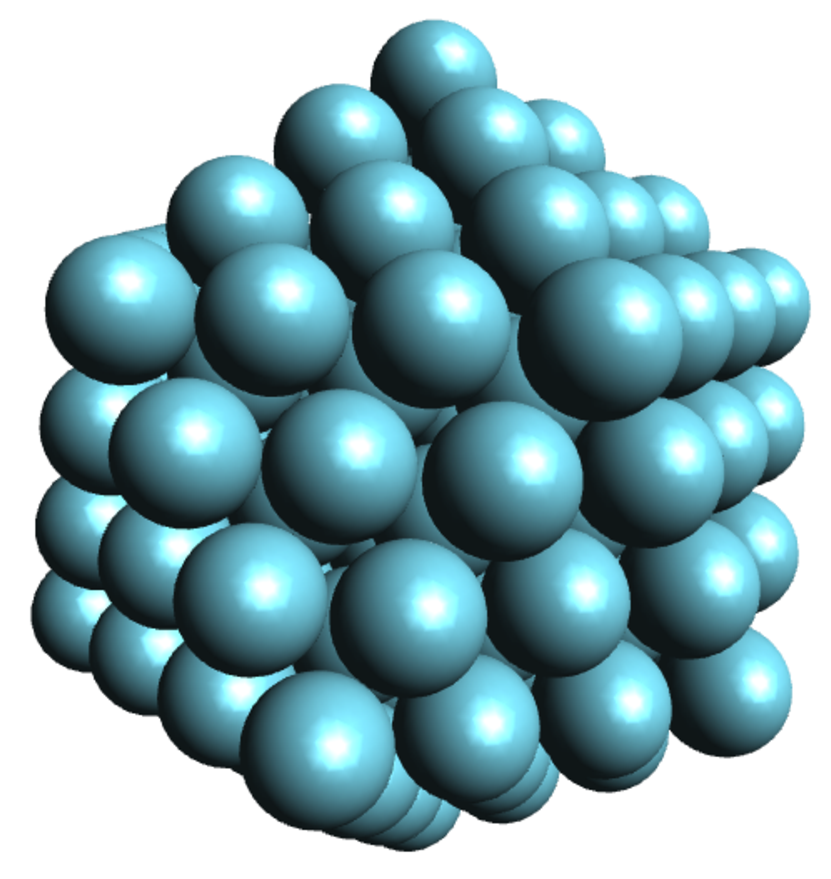
\includegraphics[scale=0.5]{pics/Ar_pure.eps}                        
 \caption{An icosahedral argon cluster with an edge consisting of 
          $c=\unit[4]{atoms}$, containing \unit[147]{atoms},
          distributed over four shells. \unit[55]{atoms} belong
          to the core, 12 are at the vertices, 60 in the edges and 20 inside the
          surfaces.}
 \label{figure:Ar_pure}
\end{figure}    

The actual cluster formation process is understood as follows. First, a three particle
collision has to take place to form argon dimers. Subsequently, single atoms are added to the dimer 
due to collisions. At a later stage these clusters can also collide to form larger clusters. This process,
called coagulation, becomes the dominant process for the formation of very large clusters. 
The experiment of Lundwall et al. \cite{Lundwall07} was interpreted to
show clusters consisting of an argon core with distinct, complete neon
shells around it, which is plausible, since according to the sum of van der Waals
energies, this should be the most stable kind of clusters.
Therefore we take this as a starting point for our considerations of the
average structure of the clusters.

In all structures considered throughout this paper we start from an icosahedral
structure of argon atoms as shown in figure \ref{figure:Ar_pure}.
In this example, it has an edge length
of $c=\unit[4]{atoms}$ and consists of $n_{Ar}=\unit[147]{atoms}$, which can be
calculated as \cite{Martin96}

\begin{equation}
  n_{atoms} = \frac{10}{3} c^3 - 5 c^2 + \frac{11}{3} c -1 .
\end{equation}

For the construction of the structure we assume the minimum
distance between two argon
atoms to be twice the van der Waals
radius of argon $r_{Ar}=$ \unit[1.88]{\AA} \cite{Bondi64}. In order to abide by this
minimum distance in the case of two atoms in a surface position in different
shells, the distance of two atoms in the edges is slightly increased.

As we are going to see in the discussion, the outcome of the experiment
can not completely be explained by an argon core surrounded by complete neon shells.
This leads us to consider other structures with an argon core somehow surrounded
by neon atoms. These we divide into three types, so that, in total, we have four
different classes of cluster structures as shown in figure \ref{figure:structures}:

\begin{enumerate}
 \item complete shells
 \item incomplete shells around complete shells
 \item caps
 \item randomly arranged neon atoms around complete shells
\end{enumerate}

\begin{figure}[!h]
 \centering
 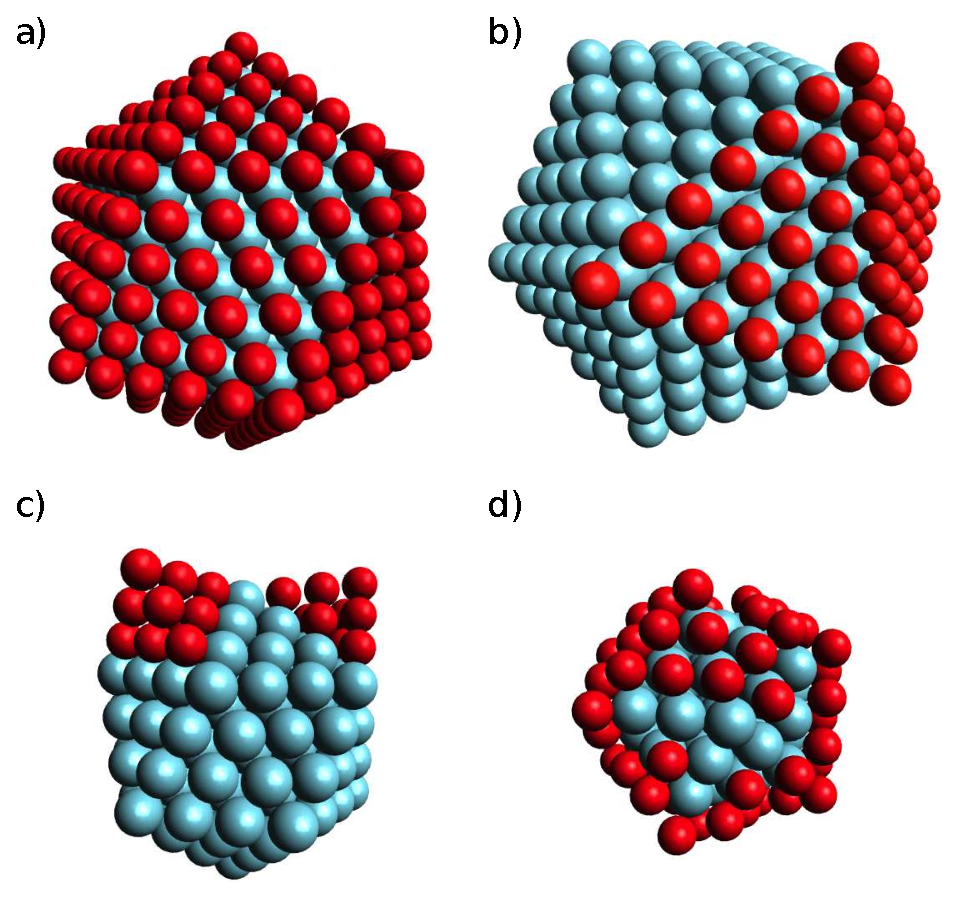
\includegraphics[scale=0.9]{pics/NeAr_structures1.eps}
 \caption{Structure classes considered in our calculations.\\
          a) complete shells, in this example $c=\unit[5]{atoms}$ with one layer
          neon atoms,\\
          b) incomplete shells, in this example
          $c=\unit[6]{atoms}$ with two covered trinangular surfaces
          of neon,\\
          c) caps, in this example $c=\unit[4]{atoms}$ with two caps,\\
          d) randomly arranged neon atoms around a full shell cluster,
          here $c=\unit[3]{atoms}$ directly covered by neon atoms
          with an argon content of \unit[47]{\%}.}
 \label{figure:structures}
\end{figure}

In the case of an argon cluster with one or more complete shells of neon
atoms around it, first the core structure is created and afterwards the
outer shells are constructed around it, such that the minimum distance between a
neon atom in the surface and an argon atom in the shell beneath is the sum
over the van der Waals radii, where $r_{Ne}=$\unit[1.54]{\AA} \cite{Bondi64}
(see figure \ref{figure:structures} panel a).

Not all experimentally determined argon contents in the mixed clusters
fit to complete neon shells. Maintaining the idea of shells,
we consider the possibility of incomplete shells.
The cluster structures are created analogously to the
complete shells except that not all triangular surfaces areas of the argon core
are covered by neon atoms (for an example see figure \ref{figure:structures}
panel b).

Another possibility are caps covering surface areas as shown
in figure \ref{figure:structures} panel c. These structural elements
do not exhibit minimum energy for clusters, but they might explain a
large number of neon-neon interactions compared to the number of
neon-argon interactions in the experiments.
The neon-neon distances within the caps are
calculated in the same
manner as described before for the (in-)complete shells.
A whole manifold of different positionings of several caps are in principle
possible, but in our calculations we were able to see, that these different
placements of caps did not change the ratios of NeAr to NeNe ICD for a
constant number of caps. Since we
are unable to distinguish these structures, we will limit ourselves to the
discussion of structures containing different numbers of caps.

One could also think about neon atoms randomly arranged around a homonuclear
or heteronuclear cluster with complete shells and randomly attached neon
atoms around it as shown in figure \ref{figure:structures} panel d.
It is constructed as a cluster with complete shells and afterwards adding
neon atoms in random positions of the next layer until the requested
$n_{Ar}/n_{Ne}$ ratio is reached.

All these structures are idealized and highly symmetric, which reduces
the computational cost. Vibrations inside the clusters will change the atom
distances and hence both the kinetic energy of the ICD electron as well as
the decay widths. As has been shown for NeAr \cite{Scheit06}, the ICD processes
are faster than dynamical rearrangements, caused by Coulombic attraction
after the initiating ionization, or vibrations. In case of the neon dimer, the
ICD lifetime is of comparable size to the rearrangement time and hence
influences the ICD electron spectra /cite{Scheit03}. However, in clusters, the
initially ionized atom interacts with more than one other atom, which leads
to more neighbors it can undergo ICD with and hence the decay width increases
to first approximation linearly with the number of nearest neighbors.
At the same time, the larger number of neighbors stabilizes the position
of the initially ionized atom in space compared to the dimer.
Therefore we will assume that the structures given above are good
approximations to the decaying clusters.




\subsection{Interpretation of the graphs}

In order to have comparable numbers we choose the argon content within
the clusters and the amount of NeAr-ICD compared to the total ICD to
characterize every measurement and theoretical calculation.
Throughout the paper, including the supplementary material, we stick to the same 
colour coding as for the experimental spectra shown in figure \ref{figure:selected_ICD_specs},
for which the numbers are listed in table \ref{table:clustervalues}.
The results are going to be plotted as in figure \ref{figure:incompl01_02_explain}.
As an example we show cluster of the class of an incompletely filled neon shell
around an argon core with a an edge size of $c=2$
surrounded by one complete shell of neon atoms.
Here the ratio of NeArICD to total ICD is plotted against the argon content
of the cluster. The results of the five different experimental conditions and their
errors are shown by the coloured areas, where the colour corresponds to the
set with the same colour as in figure \ref{figure:selected_ICD_specs}.
They are going to be the same in all plots throughout the paper.
Additionally plotted are the theoretical results for the different structures
parted into first the classes of the structures and secondly by the size of the argon core.
The higher the argon content is, the less of the 20 surfaces of the underlying
complete shell is covered by either layer(s) or caps. The easiest way to interpret
the graphs is to start from a complete shell and then covering one surface. This
corresponds to the rightmost theoretical value within a group. Each step further
to the left refers then to one more covered layer with either caps or layers.\\

\begin{figure}[!h]
  \centering
  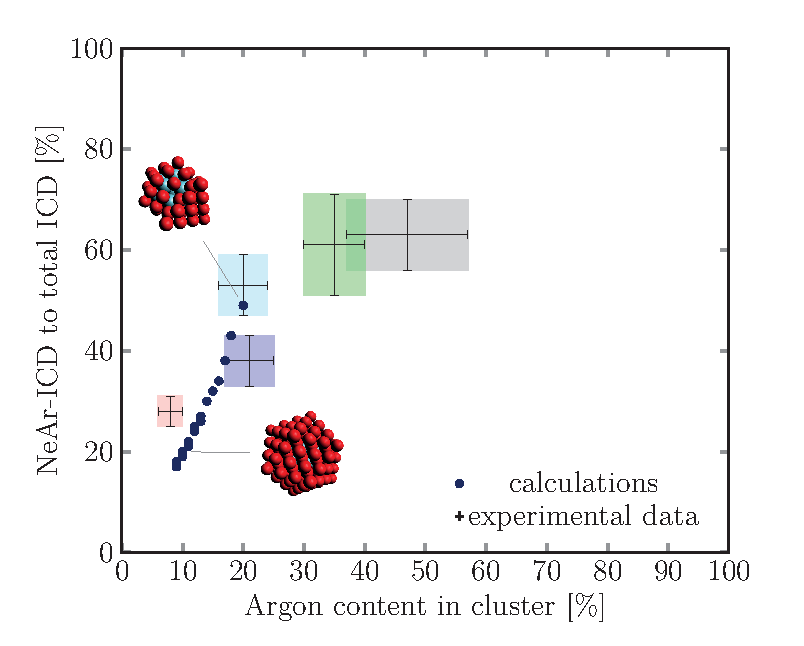
\includegraphics[scale=0.75]{pics/incompl01_02_mit_inlays.eps}
  \caption{NeArICD to total ICD ratio plotted against the argon content
           in the cluster for both experimental results for all five sets of
           conditions as well as theoretical calculations for cluster structures
           with an incomplete outermost shell surrounding an argon core of
           $c=2$ and one additional complete neon shell. For illustration, pictures
					of two structures are included at their respective theoretical values.}
  \label{figure:incompl01_02_explain}
\end{figure}

By looking for agreements of theoretical and experimental values we deduce
possible structures.
The agreement between experimental and theoretical results are evaluated
using the graphical distance from the experimental results
\begin{equation}
  d = \sqrt{\Delta_{Ar}^2 + \Delta_{\Gamma}^2}    ,
\end{equation}
where $\Delta_{Ar}$ and $\Delta_{\Gamma}$ denote the deviation of the argon content
and the ratio of NeArICD decay width and the total decay width, respectively.
Only such structures are considered, where the argon content of the model
structure lies within the error range of the experimental findings.


\subsection{Assignment of the different measurements to cluster structures}
For our assignments we use the following criteria:

\begin{itemize}
 \item onsets of single ionization potentials for the determination
       of the size of the argon core
 \item positions of NeAr-ICD peak
 \item relative expected mean cluster sizes (see table \ref{table:expansion})
 \item agreement of predicted and measured ICD (see table \ref{table:assignments})
\end{itemize}

From the onsets of the single ionization potentials and the position of the
NeAr-ICD peak at a lower energy we deduce that the mean argon core of set 5
is the smallest of all measured ensembles. Since the nearest neighbours have
the largest influence of such a shift we interprete these clusters to have
an edge length of either $c=1$ or $c=2$.\\
Since the estimation of mean cluster sizes based on Hagena refer to expansions
of only one atom type, only the results with the same argon content should
be compared. From this we expect the core of set 2 to be bigger than the core
of set 4 and the core of set 3 to be slightly larger than the core of set 1.
These estimations do not have to resemble the final conclusions, since the
approach is only valid for homogeneous clusters, but can give hints
in the following procedure. The assignment due to geometrical distance
of the predicted results from the experimental counterparts is to be found in
table \ref{table:assignments}. There best results for all sets are shown
in the following way: $c$ depicts the number of atoms in the longest edge
of the argon core, which is then covered by a number of additional complete
neon shells with additional covered triangular surfaces or randomly arranged atoms
and $d$ denotes the geometrical distance.\\

\begin{table}[!h]
  \caption{Note that for set 4 only the random arrangement is listed,
           for which the argon content exactly equals the experimental one.}
  \centering
  \begin{tabular}{lccccc}
    \toprule
     Set  & $c$ & complete Ne shells & covered surfaces & random & $d$\\
    \midrule
      1   & 4   &          1         &        1         &   -    & 2.000\\
      1   & 5   &          1         &        2         &   -    & 4.472\\
      1   & 2   &          0         &        5         &   -    & 4.472\\
    \midrule
      2   & 3   &          1         &        -         &   x    & 1.000\\
      2   & 3   &          1         &        1         &   -    & 3.162\\
      2   & 2   &          0         &        8         &   -    & 4.123\\
    \midrule
      3   & 2   &          1         &        3         &   -    & 4.000\\
      3   & 3   &          1         &        7         &   -    & 4.123\\
      3   & 3   &          1         &        8         &   -    & 4.472\\
    \midrule
      4   & 2   &          1         &        -         &   x    & 2.000\\
      4   & 2   &          1         &        1         &   -    & 4.000\\
    \midrule
      5   & 2   &          1         &       13         &   -    & 8.246\\
      5   & 2   &          1         &       14         &   -    & 9.220\\
      5   & 2   &          1         &       15         &   -    & 9.220\\
    \bottomrule
  \end{tabular}
  \label{table:assignments}
\end{table}

We are going to discuss the structure assignment in descending order
of the set number, which more or less corresponds to a discussion with
increasing size of the clusters.\\
We start our assignment with set 5 (red). As already mentioned we expect these clusters
to be small and, additionally, the smallest ones measured. These expectations are
in agreement with the results of figure \ref{figure:incompl01_02_explain}
(also to be found in the
appendix in figure \ref{incompl01_02}), where the red square
can be matched with a cluster with an argon core with $c=2$, one complete
shell of neon atoms 
and one almost complete
shell with 13 -- 20 out of 20 surfaces covered by neon atoms. None of the
theoretical estimates coincide with the experimental findings. This might be
explained by even smaller clusters not showing an icosahedral argon core, but
a coagulation of 2--11 atoms plus some neon atoms.

Set 4 (turquoise) shows a very good agreement for a structure with $c=2$ with one
complete shell of neon atoms and some additional atoms (see figures
\ref{random02} and \ref{incompl01_02} or in the example above). Whether these atoms are
randomly arranged around the complete shells or are to be found together can not
finally be decided. From the geometric distance, the random arrangement should
be preferred.

The results of set 3 (blue) shows a good agreement with structures
of $c=2$ or $c=3$ surrounded by one complete shell of neon atoms and additional
neon atoms covering 3 or 7 -- 8 triangular surfaces, respectively 
as shown in figure \ref{incompl01_02} and \ref{incompl01_03}. 

With the two latter assignments we are able to distinguish
the structures of two cluster manifolds with the same argon content by utilizing the
ICD spectra.

Set 2 (green) can be assigned to core sizes of $c=2-3$ plus further neon atoms
(see figures \ref{incompl00_02} and \ref{incompl01_03}).
In the case of $c=3$ one additional complete shell of neon atoms fits
best to the experimental results, but as for set 4 the arrangement as such for
some few additional atoms can either be random or coagulated.
In case of $c=2$ the best fit holds for no additional complete shell of
neon atoms but with 8 triangular surfaces covered, the shell is almost halfway filled.
Further structures with larger core sizes as $c=4$
are also quite probable. Considering, that 
both from Hagena's approach and considering the single ionization potential
onsets of the Ar3p band, set 2 is supposed to have the largest mean structure
core. These structures might be closer to reality than the ones of the small clusters
with $c=2,3$.

Due to the large error bars, set 1 (black) can be assigned to a whole manifold
of different structures with $c = 2 - 6$ within the error bars
either with caps or, more probably,
with about one complete shell of neon atoms, plus maybe additional covered surfaces
or randomly surrounded by neon atoms. Since caps should be energetically less
favourable than the other structures, we suspend those structures and concentrate
on the rest.
From Hagena's approach we concluded, that the core of the clusters of set 1
should be slightly
smaller or of comparable size as the clusters from set 3. Therefore we assume
the average cluster structure to consist of an argon core of $c=2-4$ shells
with one complete neon shell and possibly one further incomplete shell, of
which we can't give more detailed information.

We may have to consider completely different structures not investigated in this
paper. It might be, that formed mixed clusters collide and coagulate, yielding
structures impossible to be estimated by a core-shell structure of the kinds
presented in this paper. 

From the best agreement of the calculated NeArICD to total ICD ratios listed in table
\ref{table:assignments}, we plot the corresponding estimated spectra in figure
\ref{figure:theo_specs} folded by gaussians with a width of \unit[250]{meV}.
From these spectra and the underlying calculations
we conclude, that the shoulders of both the NeNeICD and the NeArICD peak
at \unit[2.5--4]{eV} and \unit[8--10]{eV}
correspond to next-nearest neighbours inside the clusters, while the differences
in the main peak stem from almost equal atomic distances but different positions
in the cluster such as corner, edge or surface.\\
The main peaks of the NeNeICD correspond well with the experimental observations
of figure \ref{figure:selected_ICD_specs}.\\
The onset of the NeArICD peak depends on the shielding of the argon atom
and hence the cluster size. For set 5 the assignment seems to be correct, while
for set 4, the experiment shows a higher energy of the ICD electron. 

---> den satz versteh ich nicht ganz:
This change does not need to be physical as we in the beginning assumed clusters
until $c=2$ to have the higher mean ionization potentials. 
----

The truth, however,is not a spontaneous jump from one shell to the other, but rather a decrease
with more and more atoms. If one is interested in clusters of $c\le2$ only, one
should take care of a more detailed description of the different ionization
potentials for different cluster sites.\\

\begin{figure}[!ht]
  \centering
      \begin{tikzpicture}

        \begin{axis}[
            use units,
            x unit=eV,
            y unit=a.u.,
%            title={Spektrum},
            xmin=0,
            xmax=10.5,
            axis x line=bottom,
%            axis x discontinuity=parallel,
            ymin=0,
            ymax=3.4,
            axis y line=left,
            samples=1000,
            scale=0.55,
            legend style={draw=none},
            legend cell align=center,
            legend pos=outer north east
            ]

        \addplot[
            mark=none,
            color=black,
            ]
            table[
            x expr=\thisrowno{0},
            y expr=\thisrowno{1} * 25.4518
            ]
            {data/near_clusters/set1.sp};
        \addplot[
            mark=none,
            color=green,
            ]
            table[
            x expr=\thisrowno{0},
            y expr=\thisrowno{1} * 27.0625
            ]
           {data/near_clusters/set2.sp};

        \addplot[
            mark=none,
            color=blue,
            ]
            table[
            x expr=\thisrowno{0},
            y expr=\thisrowno{1} * 43.2460
            ]
            {data/near_clusters/set3.sp};

        \addplot[
            mark=none,
            color=cyan,
            ]
            table[
            x expr=\thisrowno{0},
            y expr=\thisrowno{1} * 35.4689
            ]
            {data/near_clusters/set4.sp};

        \addplot[
            mark=none,
            color=red,
            ]
            table[
            x expr=\thisrowno{0},
            y expr=\thisrowno{1} * 76.3945
            ]
            {data/near_clusters/set5.sp};
        \end{axis}
    \end{tikzpicture}


  \caption{Calculated ICD electron spectra for those structures given in table
           \ref{table:assignments} with the best agreement to the experimental
           argon content and NeArICD to total ICD ratio. The intensities are given
           in arbitrary units and are normalized to the peak height of the NeArICD
           peak and the spectra are folded by Gaussians with widths of \unit[250]{meV}.
           The theoretically calculated specrta nicely match the experimental ones in figure
           \ref{figure:selected_ICD_specs}.
           Both, the NeNeICD peak at low energies and the NeArICD peak
           at higher kinetic energies, show a peak structure which can be related
           to different distances of the atoms involved in the process within the
           clusters. For more details, see the text.}
  \label{figure:theo_specs}
\end{figure}


